\item 
\begin{enumerate}
    \item[(a)] Demuestre que el volumen de un segmento de altura $h$ de una esfera de radio $r$ es
    $$V = \frac{1}{3}\pi h^2(3r - h)$$
    \item[(b)] Demuestre que si una esfera de radio 1 se corta por un plano a una distancia $x$ del centro, de manera que el volumen de un segmento sea el doble del otro, entonces $x$ es solución de la ecuación
    $$3x^3 - 9x + 2 = 0$$
    en donde $0 < x < 1$. Utilice el método de Newton para encontrar $x$ con una exactitud de cuatro cifras decimales.
    \item[(c)] Mediante el uso de la fórmula del volumen del segmento de una esfera, se puede demostrar que la profundidad $x$ a la que se sumerge una esfera flotante de radio $r$ en el agua es una raíz de la ecuación
    $$x^3 - 3rx^2 + 4r^3s = 0$$
    en donde $s$ es la densidad relativa de la esfera. Supóngase que una esfera de madera de radio $0.5 \text{ m}$ tiene una densidad relativa de $0.75$. Calcule, con una exactitud de cuatro cifras decimales, la profundidad a la que se sumergirá la esfera.
    \item[(d)] Un tazón hemisférico tiene un radio de $5 \text{ pulg}$ y fluye agua hacia su interior a razón de $0.2 \text{ pulg}^3/\text{s}$.
    (i) ¿A qué velocidad aumenta el nivel del agua en el tazón en el instante en que la profundidad es de $3 \text{ pulg}$?
    (ii) En cierto instante, el agua tiene $4 \text{ pulg}$ de profundidad. ¿En cuánto tiempo se llenará el tazón?
\end{enumerate}
\begin{center}
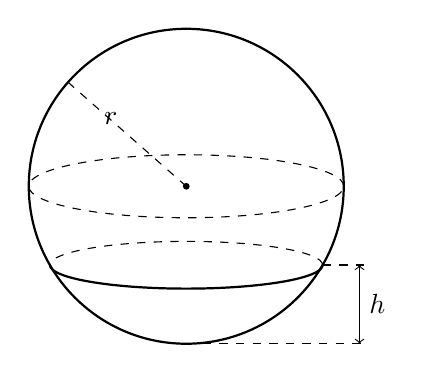
\begin{tikzpicture}[scale=1]
    \draw[thick] (0,0) circle (2cm);
    \draw[dashed] (0,0) ellipse (2cm and 0.4cm);
    \draw[thick] (-1.732,-1) arc (180:360:1.732cm and 0.3cm);
    \draw[dashed] (1.732,-1) arc (0:180:1.732cm and 0.3cm);
    \draw[dashed] (0,0) -- (-1.5, 1.32) node[midway, above left] {$r$};
    \draw[<->] (2.2, -2) -- (2.2, -1) node[midway, right] {$h$};
    \draw[dashed] (0,-2) -- (2.3,-2);
    \draw[dashed] (1.732,-1) -- (2.3,-1);
    \filldraw (0,0) circle (1pt);
\end{tikzpicture}
\end{center}
